\documentclass[final,hyperref={pdfpagelabels=false}]{beamer}
\mode<presentation>{\usetheme{Insight}}

% To install ubuntu fonts in LaTeX:
% https://github.com/tzwenn/ubuntu-latex-fonts
%
\usepackage{ubuntu}

% Set Size of poster with size= property: a1, a2, a3 debug
\usepackage[orientation=portrait,size=a0,scale=1.2]{beamerposter}

% Required Packages:
\usepackage{amsmath,amsthm, amssymb, latexsym}
%\boldmath
\usepackage[english]{babel}
\usepackage[utf8]{inputenc}
\usepackage{tikz}
\usepackage{graphics}
\usepackage{overpic}
\usepackage{ragged2e}
\usepackage{tcolorbox}
\tcbuselibrary{skins}
\usetikzlibrary{shadings}
\usepackage{tikz}
\usetikzlibrary{positioning}
\usepackage{tikz}
\usepackage{colortbl}
\usepackage{longtable}
\usepackage{qrcode}
\usepackage{subfigure}
\usepackage{booktabs}
\usepackage{multirow}
\usepackage{multicol}
\setlength\columnsep{1.4cm}
\usepackage{hyperref}



%%%% replace as required
\title{Developing training courses on AI and\\Combinatorial Optimisation for the ENTIRE EDIH}
\author{Helmut Simonis, Liam O'Toole, Luis Quesada, and Kristin Bracewell}
\institute[Insight]{Insight Research Ireland Centre for Data Analytics, School of Computer Science and Information Technology\\University College Cork\\Cork, Ireland}

\date{}
%%%%%%%%%%%%%%%%%%%%%%%%%%%%%%%%%%%%%%%%%%%%%%%%%%%%%%%%%%%%%%%%%%%%%%%%%%%%%%
\begin{document}
\begin{frame}{}
%%%%%%%%%%%%%%%%%%%%%%%%%%%%%%%%%%%%%%%%%%%%%%%%%%%%%%%%%%%%%%%%%%%%%%%%%%%%%%

\begin{multicols}{3}

\section{Key Points}

\begin{itemize}
\item Three courses on AI and optimisation
\item Intended for SME and public PSO
\item One or two day (scheduling), in person courses
\item Focused on what can be achieved
\item Mainly using case studies from Insight/UCC
\item Developing open-source demonstrators for different applications
\item Feedback from attendees very positive
\item But, hard to reach target audience
\end{itemize}


\section{ENTIRE EDIH}


\includegraphics[width=0.3\textwidth]{images/entirepartners}

\begin{itemize}
\item European Digital Innovation Hubs (EDIH) program
\item ENTIRE focused on Munster
\item Funded by European Commission through Enterprise Ireland
\item Provide upskilling for SME and PSO through "de minimis" funding
\end{itemize}


\includegraphics[width=0.3\textwidth]{images/entirefunders}


\section{Scheduling and Planning}


\subsection{Topics}

\begin{itemize}
\item Background/Motivation
\item Scheduling Concepts
\item Machine Constraints
\item Costs and Objectives
\item Advanced Concepts
\item Case Studies
\item Literature Review
\end{itemize}


\subsection{Scheduling Tool}

\begin{itemize}
\item Open-source, generic scheduling tool
\item Problem data/results as JSON file
\item Connects to commercial and open-source solvers
\item Programmed in Java and JavaFx
\end{itemize}

\subsubsection{Gantt Chart Display}
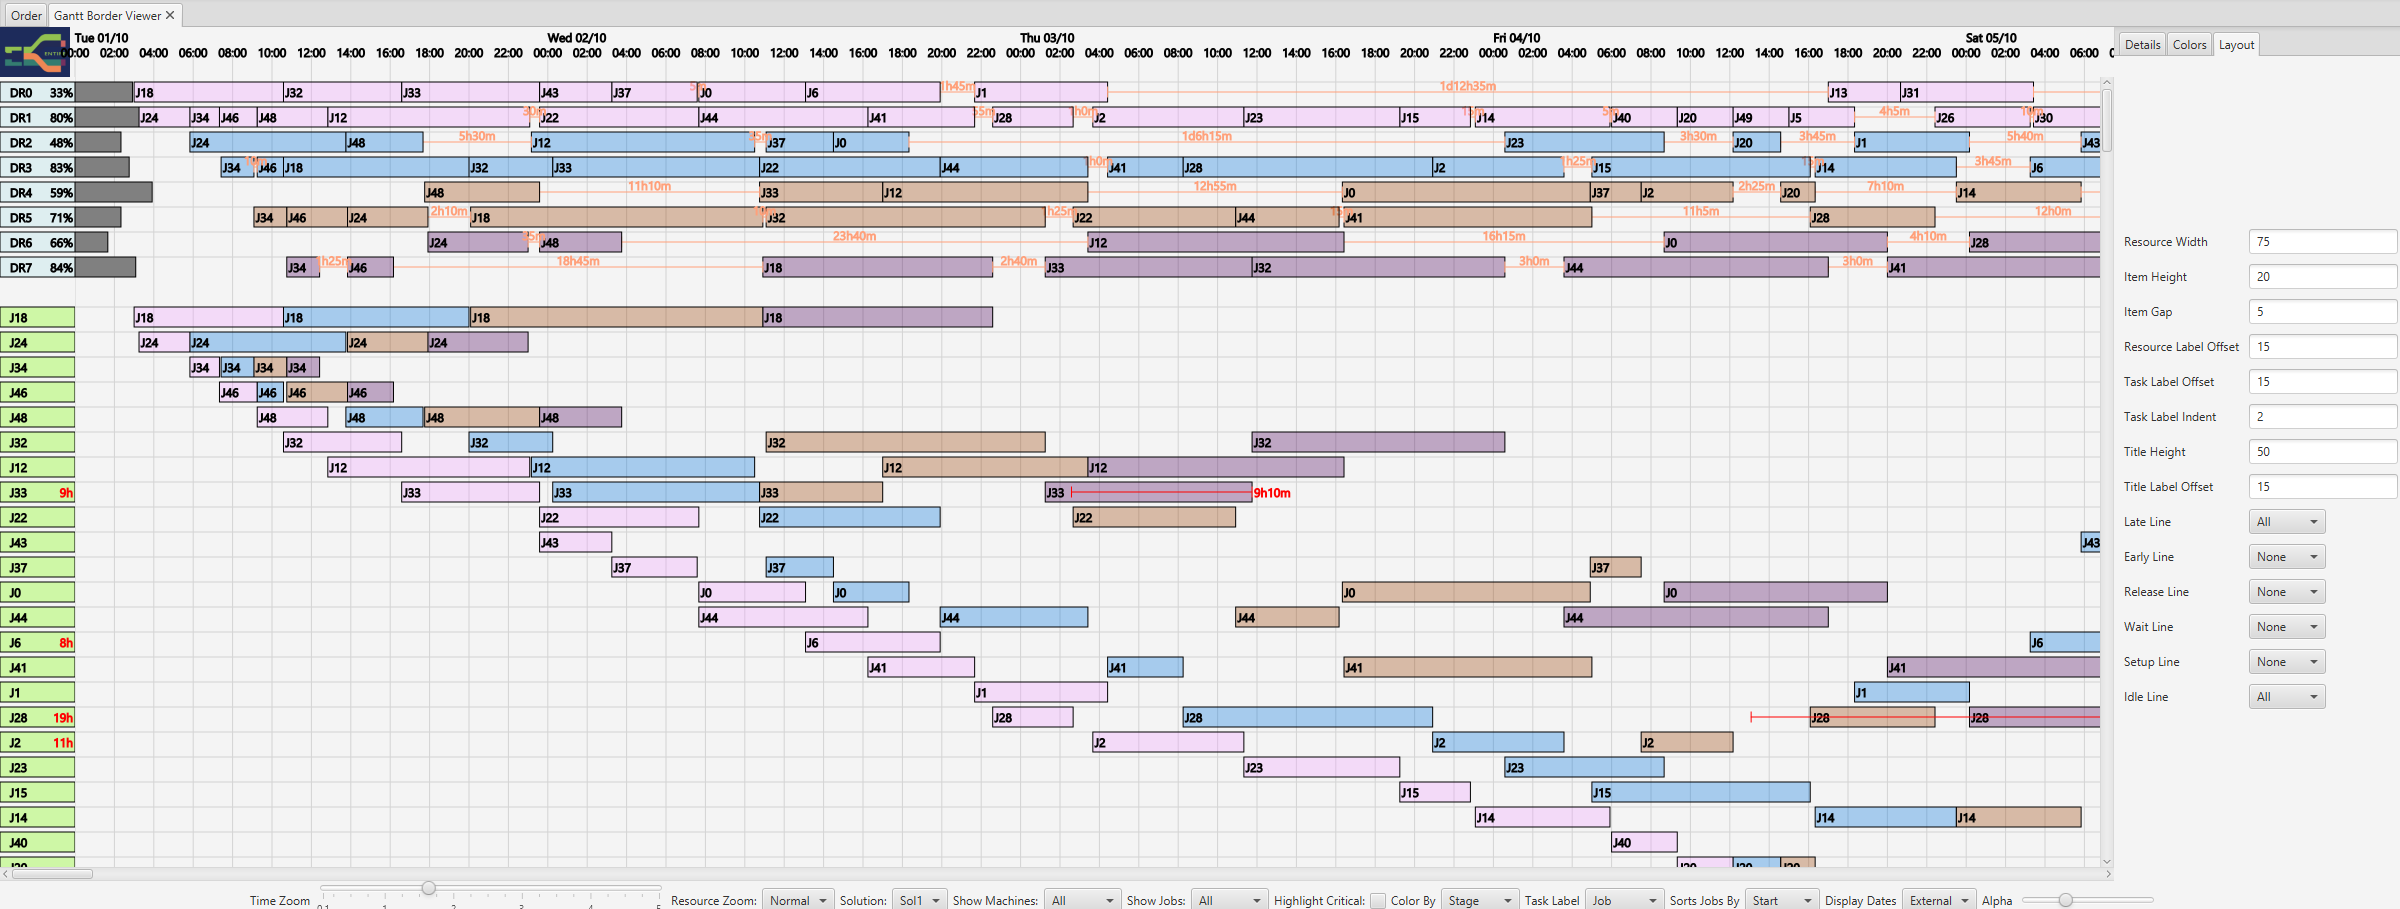
\includegraphics[width=.3\textwidth]{images/gantt-adapted}

\subsubsection{Underlying Domain Model}
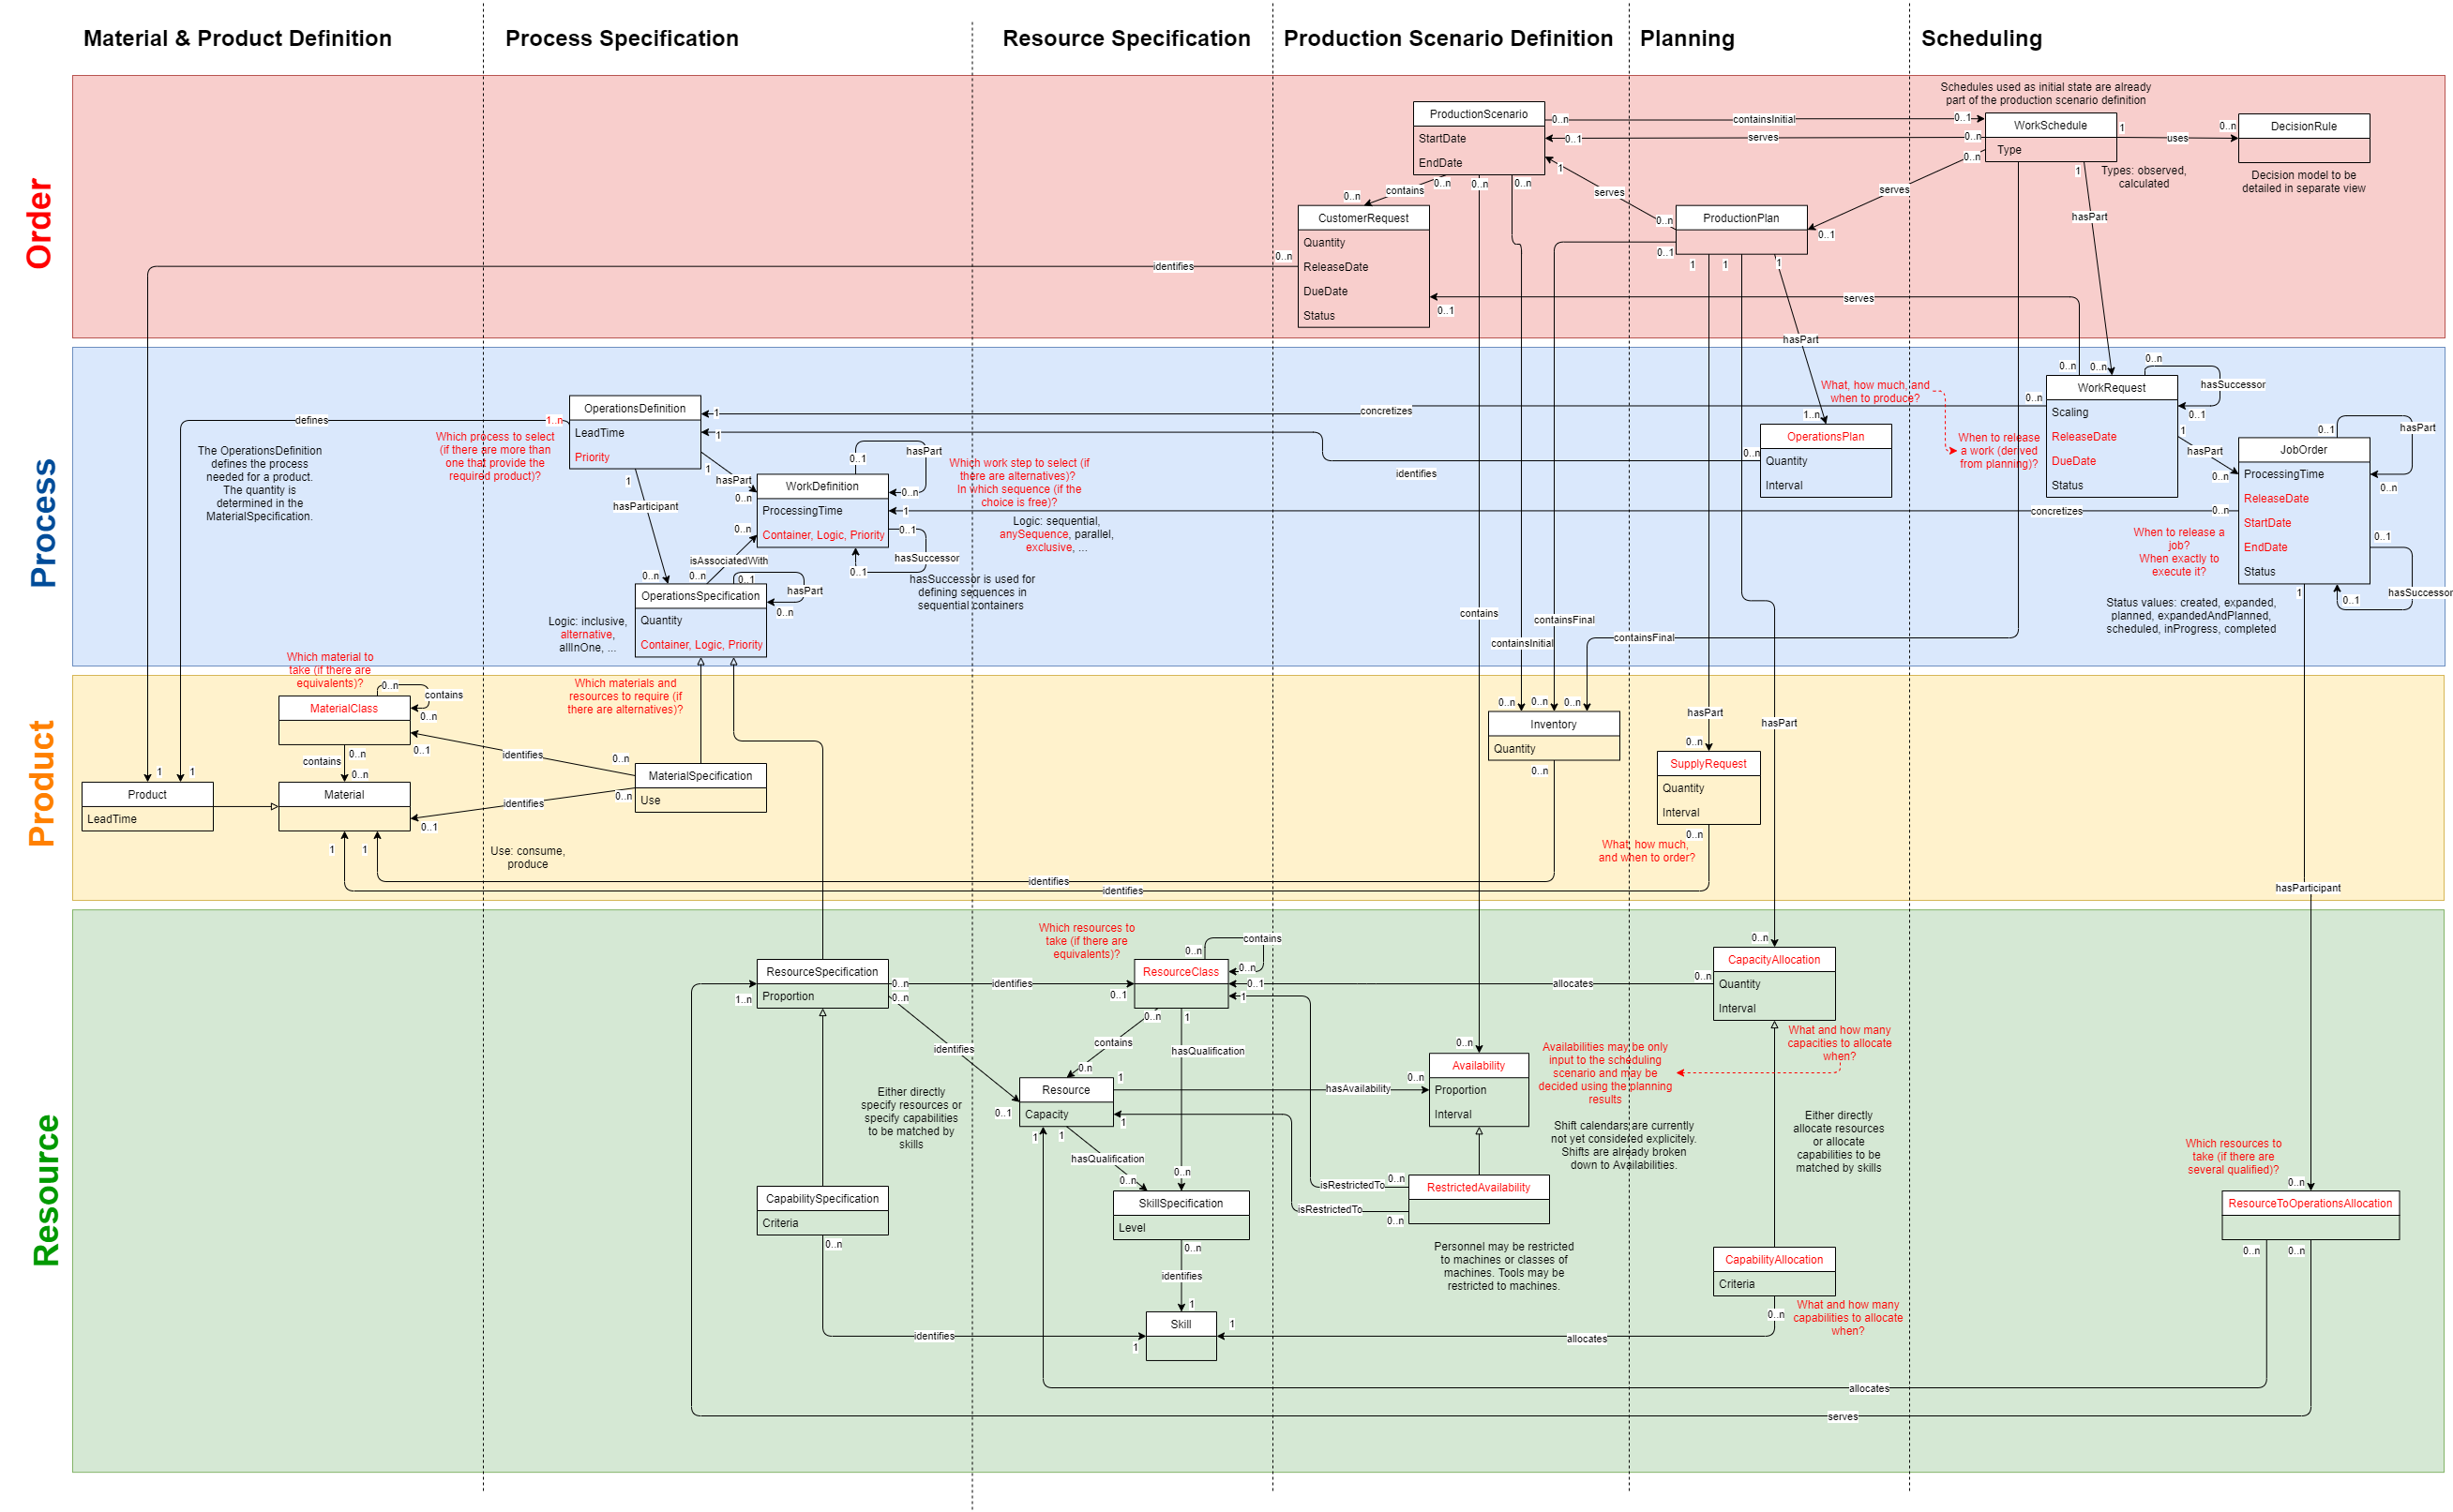
\includegraphics[width=.3\textwidth]{images/DomainModel}


\subsection{Case Studies}

\begin{itemize}
\item Production Planning
\begin{itemize}
\item Using Scheduling as a module
\end{itemize}
\item Oven Scheduling
\begin{itemize}
\item Unconventional resource constraints
\end{itemize}
\item Blades and Vanes Production Planning
\begin{itemize}
\item Multi-year scheduling for capacity planning
\end{itemize}
\end{itemize}

\subsubsection{Blades and Vanes Problem}
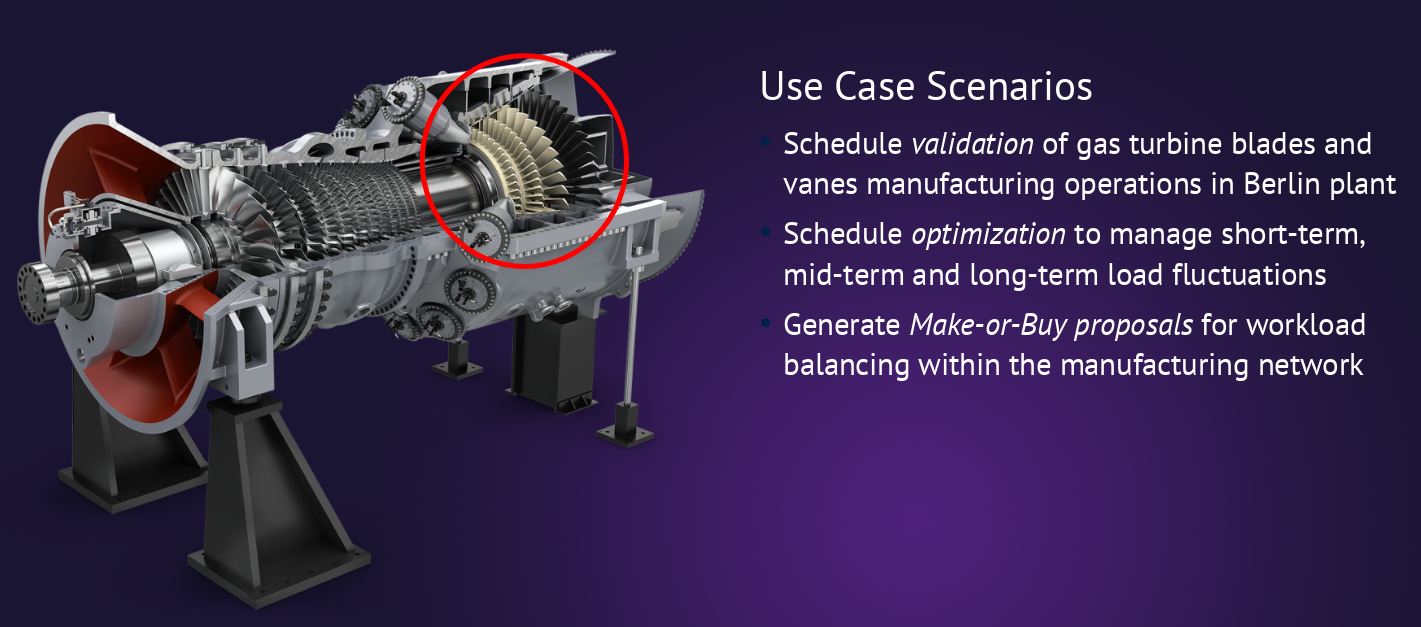
\includegraphics[width=.3\textwidth]{images/assistantgasturbine}

\section{Rostering and Timetabling}


\subsection{Topics}

\begin{itemize}
\item Introduction
\item AI and Constraint Programming
\item Rostering
\item Timetabling
\item Case Studies
\item Literature Survey
\end{itemize}

\subsubsection{UCC's Dental School Timetabling}
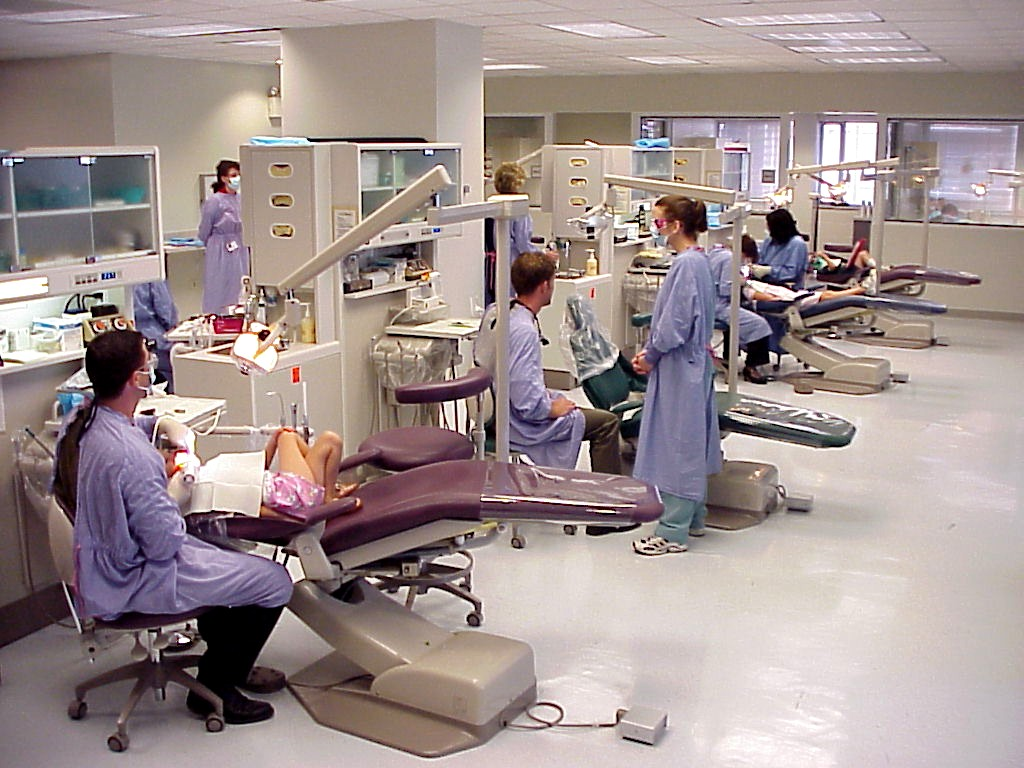
\includegraphics[width=.3\textwidth]{images/clinic.jpg}

%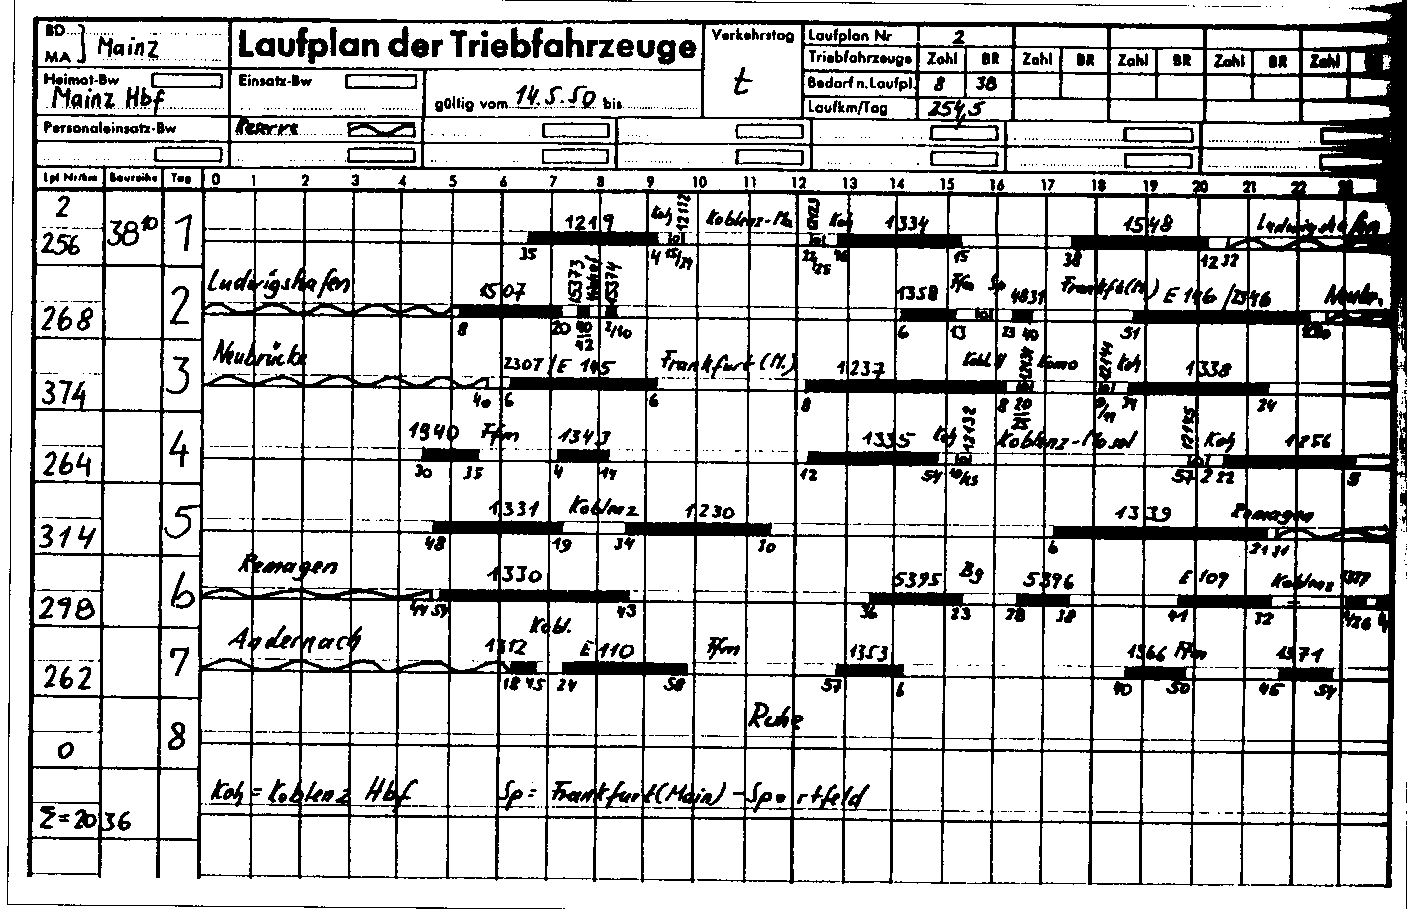
\includegraphics[width=.3\textwidth]{images/laufplancrop.png}


\subsection{Case Studies}

\begin{itemize}
\item Outpatient Waitlist Management
\item Elevator Maintenance Planning and Scheduling
\item Car Transportation
\item Yearly Rostering for Irish Naval Service
\item Catering Crew for TGV
\item Rostering for TV/Radio Stations
\end{itemize}

\subsubsection{Clustering and Route Planning}
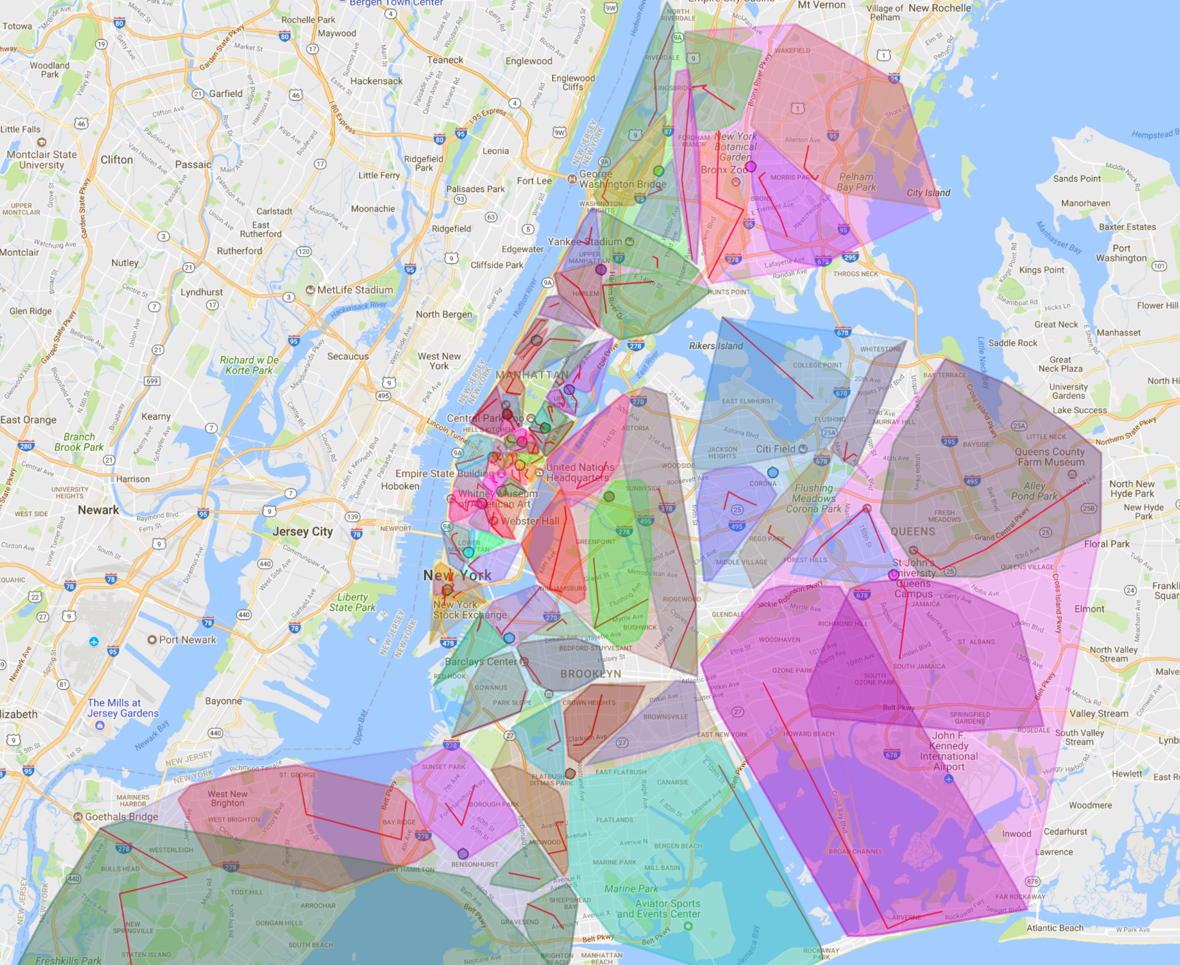
\includegraphics[width=.3\textwidth]{images/toursinroutes}



\section{Energy Cost Optimisation}



\subsection{Topics}

\begin{itemize}
\item Irish/EU Energy Market
\item Data Analysis
\item Load and Price Prediction
\item Exploiting Renewables
\item Literature Survey
\end{itemize}

\subsubsection{Predicting UCC's Electricity Consumption}
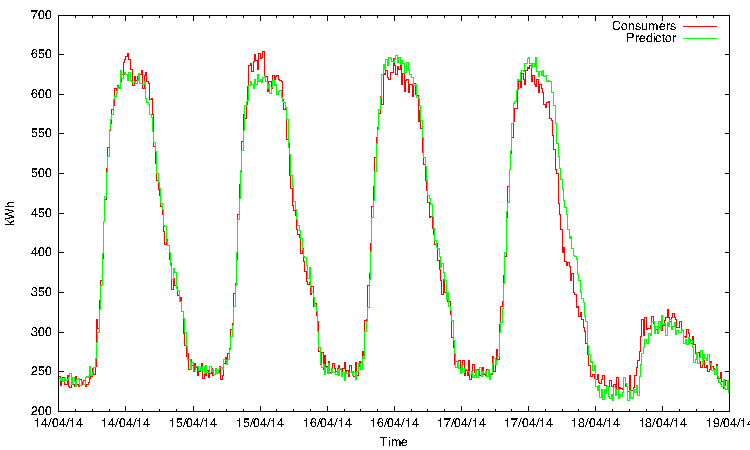
\includegraphics[width=.3\textwidth]{images/Consumers.pdf}


\subsection{Case Studies} 

\begin{itemize}
\item Anomaly detection in induction motors
\item Load forecasting in data centres
\item SEM/I-SEM Electricity price prediction
\item Scheduling UCC's CHP plant
\item Feed-mill scheduling for minimising energy cost
\item Tara mines dewatering
\end{itemize}

\subsubsection{Mine Dewatering Problem}
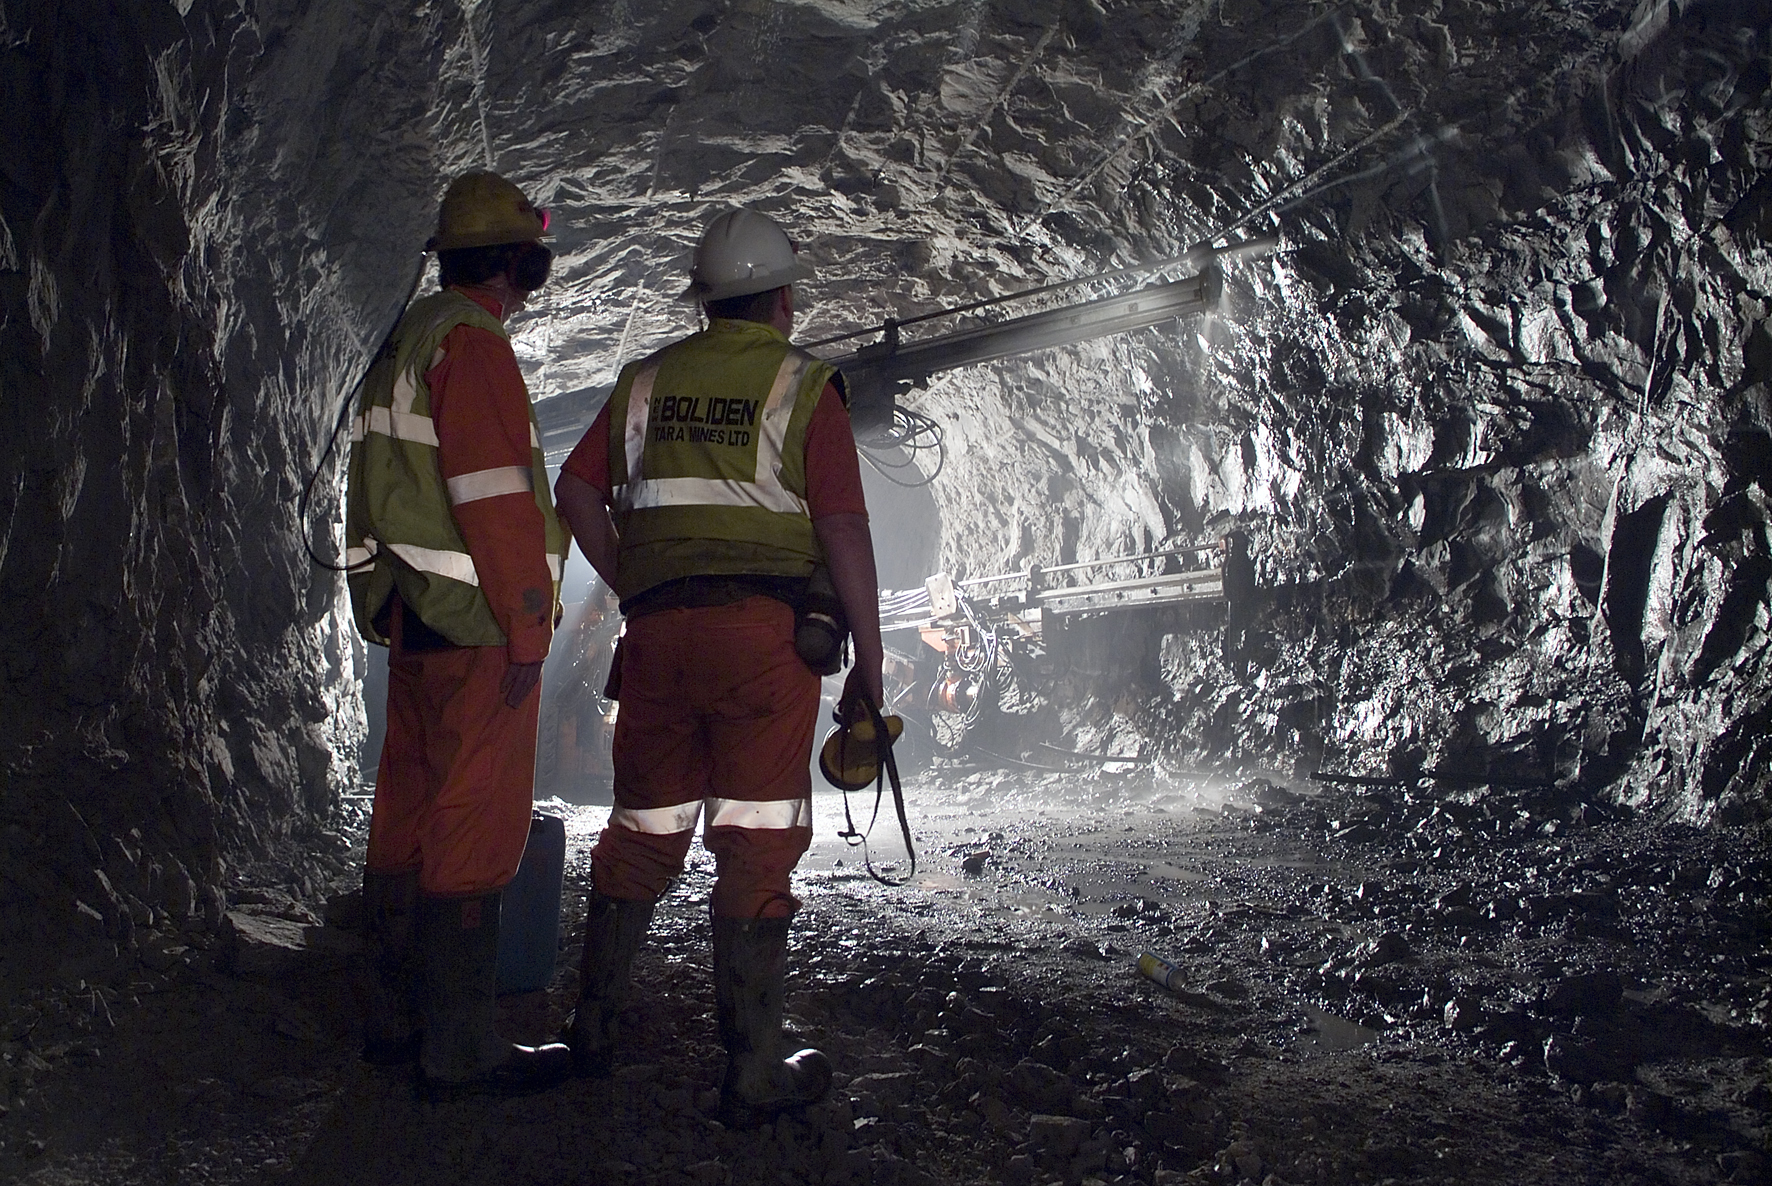
\includegraphics[width=.3\textwidth]{images/underground2}


\section{Course Delivery}
\begin{itemize}
\item Scheduling (3x)
\item Energy Cost Optimisation (2x)
\item Rostering and Timetabling (once)
\end{itemize}
Planning repeat runs in 2026
\begin{itemize}
\item One-day version of scheduling course
\item Split rostering and timetabling into separate courses
\end{itemize}


\section{To learn more}
\href{https://entire-edih.ie/}{ENTIRE Website}
\begin{center}
%%%% replace as required with more specific links
\qrcode[link,height=5cm]{https://entire-edih.ie/}
\end{center}



\end{multicols}
\end{frame}
\end{document}
%%%%%%%%%%%%%%%%%%%%%%%%%%%%%%%%%%%%%%%%%%%%%%%%%%%%%%%%%%%%%%%%%%%%%%%%%%%%%%